\section{Cloud-Side Predictive Planning}

\subsection{Traffic Graph Representation}

Cloud-side predictive planning must reason over a larger spatial range than vehicle-side local perception. In the highway scenarios considered here, a passenger car traveling at 120 km/h can cover about 667 m within 20 s. Therefore, the cloud uses a road-centered graph representation rather than a BEV raster. A large BEV image wastes computation on non-road regions, lets irrelevant background semantics dominate the representation at large spatial scales, and may confuse overlapping ramps or viaducts after projection onto a plane. A graph representation stores only reachable road elements, preserves topological connectivity, and scales with the number of road nodes rather than image area, as illustrated in Fig.~\ref{fig:graph_representation}.

\begin{figure}[t]
  \centering
  \subfloat[BEV representation issue\label{fig:bev_problem_journal}]
    {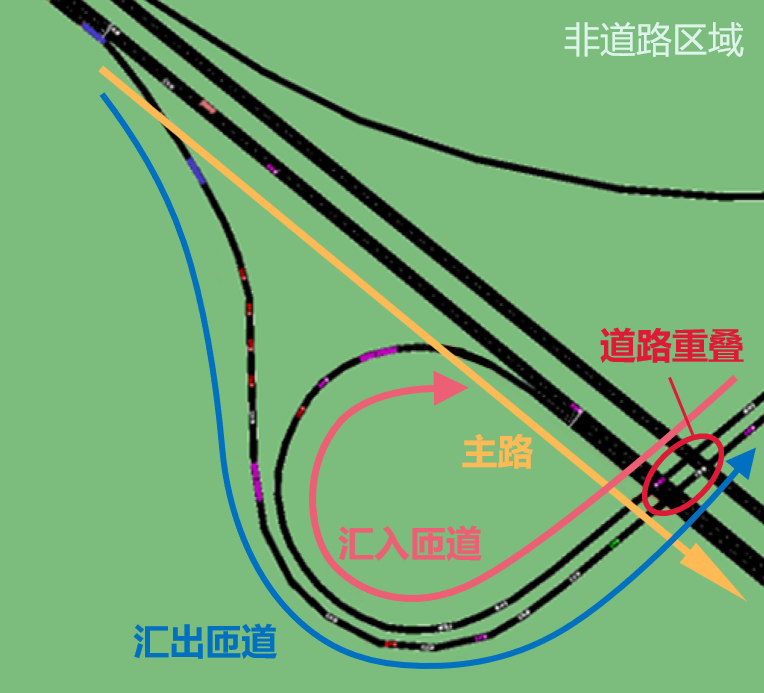
\includegraphics[width=0.44\linewidth]{fig/chap3/bev_problem.png}}
  \subfloat[Directed road graph\label{fig:graph_solution_journal}]
    {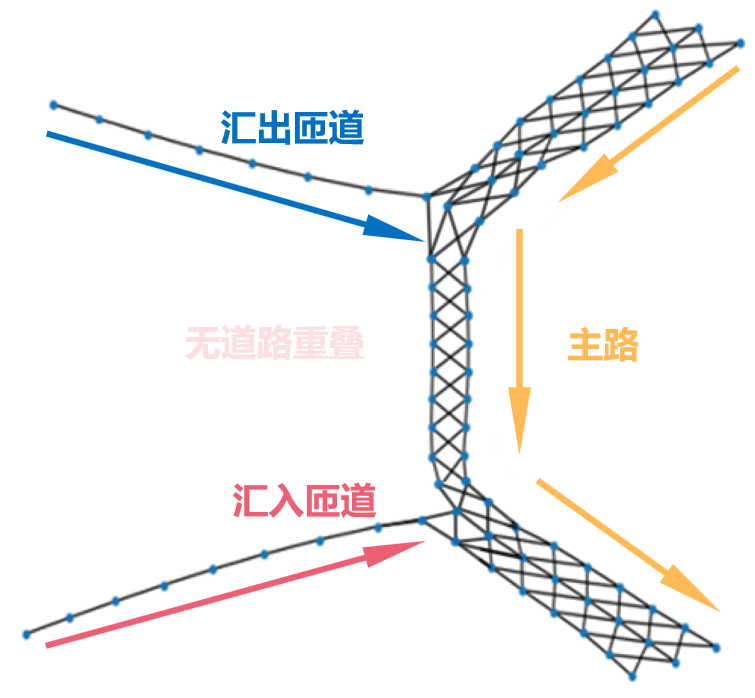
\includegraphics[width=0.44\linewidth]{fig/chap3/graph_solution.png}}
  \caption{Motivation for traffic graph representation in cloud-side predictive planning.}
  \label{fig:graph_representation}
\end{figure}

The road topology is discretized into directed road nodes. For lane-level highway modeling, each lane is discretized longitudinally and laterally, with topology-dependent connections for normal lane sections, merging/diverging sections, and junctions. The resulting graph is
\begin{equation}
  \mathcal{G}=(\mathcal{V},\mathcal{E}),\quad
  \mathcal{V}=F_{stat}\oplus F_{dyn},\quad
  \mathcal{E}=F_{con},
  \label{eq:traffic_graph}
\end{equation}
where $F_{stat}$ contains static road attributes and $F_{dyn}$ contains dynamic traffic attributes. The static node features include node position, lane position type, lane index, edge type, speed limit, and navigation-route indicator. The dynamic node features include surrounding-vehicle occupancy, vehicle type, speed, acceleration, heading, ego occupancy, estimated intention, and a risk-field value. The edge features encode connection type and normalized node distance. Fig.~\ref{fig:graph_features} shows an example.

\begin{figure}[t]
  \centering
  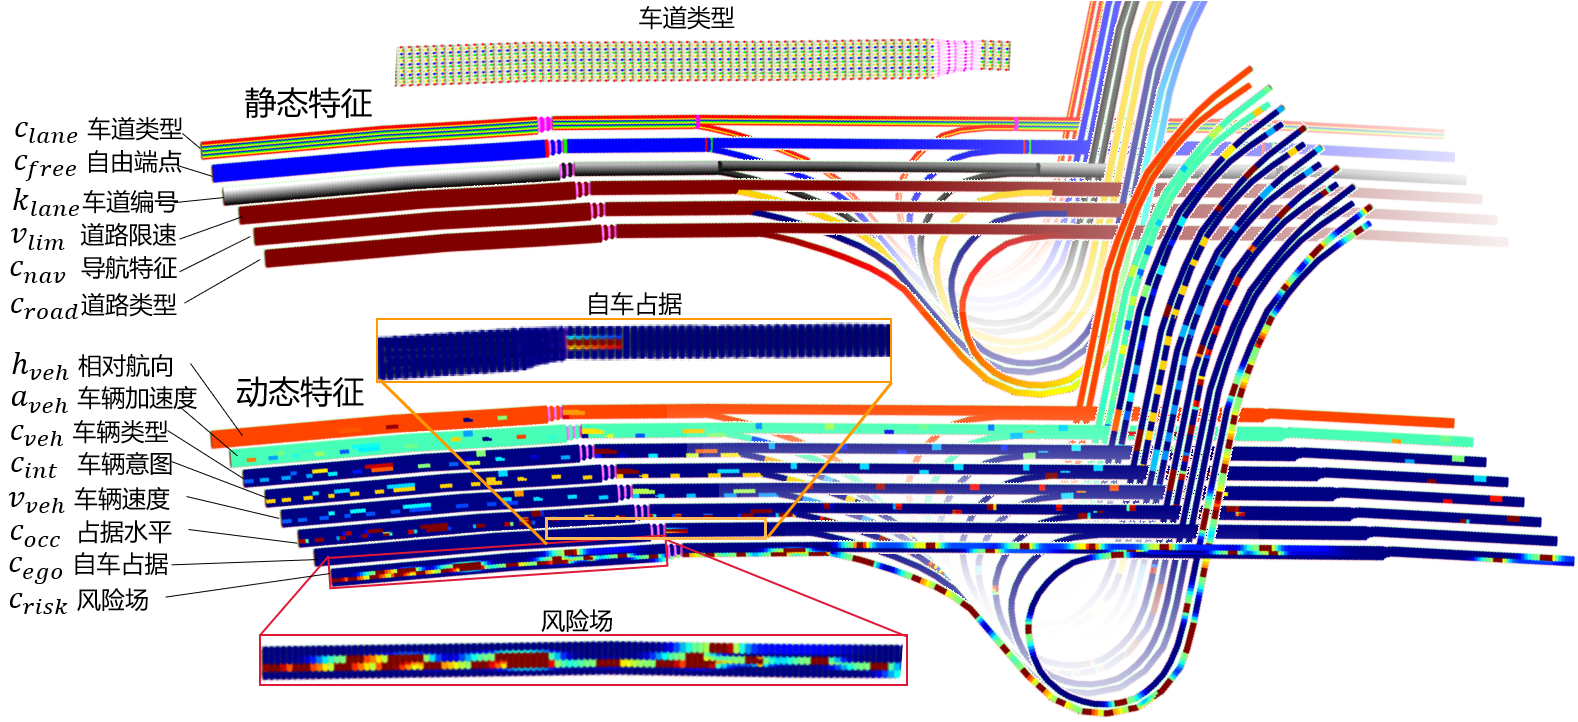
\includegraphics[width=0.95\linewidth]{fig/chap3/feature_example.png}
  \caption{Road-node and edge feature representation for the traffic graph.}
  \label{fig:graph_features}
\end{figure}

The risk field is used to provide a compact local safety prior on the graph. For node $i$ and its longitudinal neighbor $i+k$ in the same lane, the occupancy and speed risks are diffused along forward and backward graph directions:
\begin{equation}
R_{occ}(i,k)=
\begin{cases}
c_{occ}(i)\lambda_f^k, & k>0,\\
c_{occ}(i), & k=0,\\
c_{occ}(i)\lambda_b^{-k}, & k<0,
\end{cases}
\label{eq:r_occ}
\end{equation}
\begin{equation}
R_{spd}(i,k)=
\begin{cases}
c_v^+(i)\lambda_f^k, & k>0,\\
c_v^+(i)+c_v^-(i), & k=0,\\
c_v^-(i)\lambda_b^{-k}, & k<0,
\end{cases}
\label{eq:r_spd}
\end{equation}
where $\lambda_f$ and $\lambda_b$ are exponential decay factors, and $c_v^+$ and $c_v^-$ are normalized relative-speed risk components. The final risk field of target node $j$ is
\begin{equation}
  \begin{aligned}
  c_{risk}(j)=\min\bigg(&
  \sum_{i\in\Omega_b(j)} R_{occ}(i,j-i)\\
  &+\lambda_{spd}R_{spd}(i,j-i),\,1\bigg),
  \end{aligned}
  \label{eq:risk_field}
\end{equation}
where $\Omega_b(j)$ is the set of same-lane source nodes that can contribute risk to node $j$.

\subsection{Graphflow-Based Interactive Prediction}

Graphflow is designed as an autoregressive graph-flow prediction model for long-horizon stochastic interaction. Given historical graph states, the ego action, and time encoding, it predicts the future evolution of dynamic node features over a horizon of 20 s. Unlike deterministic trajectory predictors, Graphflow models how occupancy and risk diffuse over the graph, which is more suitable for cloud-side risk anticipation than precise single-trajectory prediction at long horizons. This formulation also avoids explicitly enumerating all surrounding-vehicle intention combinations, whose strategy tree grows rapidly with the number of vehicles and the decision horizon.

\begin{figure}[t]
  \centering
  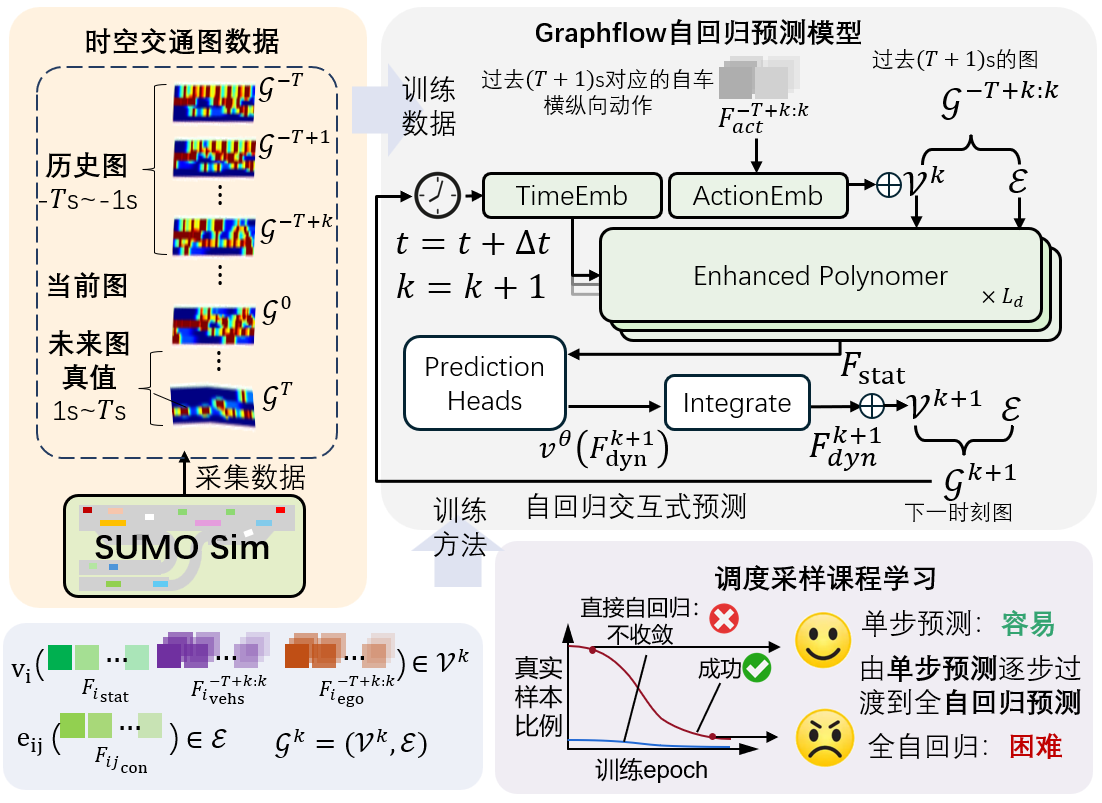
\includegraphics[width=0.95\linewidth]{fig/chap3/graphflow_training.png}
  \caption{Graphflow training and autoregressive graph diffusion.}
  \label{fig:graphflow_training_journal}
\end{figure}

The model input at step $k$ is a spatiotemporal graph
\begin{equation}
  \mathcal{G}_{st}^{k}=
  \left\{F_{stat},F_{dyn}^{k-T:k},\mathcal{E},a_e^k\right\},
  \label{eq:graphflow_input}
\end{equation}
where $a_e^k$ is the ego action used to condition surrounding-vehicle evolution. The graph encoder contains local edge-aware graph attention for neighbor interaction and a global graph attention block for long-range dependency. Time and ego-action encodings are injected into node embeddings. The model outputs a velocity field of dynamic node features:
\begin{equation}
  v_t^{\boldsymbol{\theta}}(F_{dyn}^{t}|\mathcal{G}_{st}^{k}),
  \quad t\in[k,k+1].
  \label{eq:graphflow_velocity}
\end{equation}

The flow-matching objective is used because the training data contain true graph evolution between adjacent time steps. A target velocity field $v_t^{target}$ is obtained by time interpolation and differentiation between $F_{dyn}^k$ and $F_{dyn}^{k+1}$. The conditional flow-matching loss is
\begin{equation}
  \mathcal{L}_{CFM}(\boldsymbol{\theta})=
  \left\|
  v_t^{\boldsymbol{\theta}}(F_{dyn}^{t}|\mathcal{G}_{st}^{k})
  -v_t^{target}(F_{dyn}^{t}|F_{dyn}^{k+1})
  \right\|_2^2.
  \label{eq:cfm_loss}
\end{equation}
The predicted next graph is obtained with one-step numerical integration:
\begin{equation}
  F_{dyn}^{\boldsymbol{\theta},k+1}
  =F_{dyn}^{k}
  +\Delta t\,
  v_t^{\boldsymbol{\theta}}(F_{dyn}^{t}|\mathcal{G}_{st}^{k}).
  \label{eq:graphflow_euler}
\end{equation}
To reduce autoregressive drift, scheduled sampling curriculum learning is adopted \cite{DCRNN2018}. With mini-batch count $N_{batch}$, the teacher-forcing probability is
\begin{equation}
  \epsilon_{SSCL}=
  \frac{\tau_{SSCL}}
  {\tau_{SSCL}+\exp(N_{batch}/\tau_{SSCL})},
  \label{eq:sscl}
\end{equation}
so the model gradually shifts from ground-truth future inputs to its own predicted graph states during training.

\subsection{Long-Horizon Decision-Making}

The cloud-side decision maker uses Graphflow as a learned world model. During training, Graphflow rolls out the traffic graph under candidate ego actions and provides the predicted risk fields used by the reward. During online operation, the trained policy is executed in a receding-horizon manner. Its role is not to directly actuate the vehicle, but to determine a long-horizon behavior guide that reduces interaction-induced rollover triggers. The policy receives the current traffic graph, historical surrounding-vehicle features, and ego features. The ego features include route distance, lane and ramp attributes, ego velocity and heading, lane-change status, neighbor-risk indicators, and navigation intention. Surrounding-vehicle features include existence, relative position, relative velocity, heading, lane relation, vehicle type, route intention, and surrogate safety indicators.

The action is a sequence of acceleration and lane-change commands,
\begin{equation}
  A_c^{k:k+H_c}
  =
  \{a_{des}^{k:k+H_c},\,l_{cmd}^{k:k+H_c}\},
  \label{eq:cloud_action}
\end{equation}
where $l_{cmd}$ is represented continuously during training and mapped to lane-keeping, left-lane-change, or right-lane-change decisions during execution. Surrounding-vehicle parameter and intention uncertainty is estimated from historical cloud twin data using driver and lane-change models. The longitudinal behavior uses a differentiable IDM form \cite{IDM_2020}, while the lane-change probability follows a MOBIL-style utility model \cite{MOBIL_1999}. Bayesian sampling updates the uncertainty of these parameters and intentions when sufficient history or lane-change events are observed.

The policy is trained with PPO. Its reward combines safety, efficiency, comfort/economy, temporal consistency, traffic-rule compliance, and navigation consistency:
\begin{equation}
  r=w_s r_s+w_e r_e+w_c r_c+w_{con}r_{con}+w_r r_r+w_n r_n.
  \label{eq:cloud_reward}
\end{equation}
The safety reward integrates the risk field over ego-occupied nodes and the prediction horizon:
\begin{equation}
  \begin{aligned}
  r_s=&-\frac{1}{H_c Z_o}
  \sum_{t=1}^{H_c}\sum_{\mathbf{v}\in\mathcal{V}}
  \gamma^t c_{risk}(\mathbf{v},t)\mathbb{I}(c_{ego}>\epsilon_o),\\
  Z_o=&\sum_{\mathbf{v}\in\mathcal{V}}\mathbb{I}(c_{ego}>\epsilon_o).
  \end{aligned}
  \label{eq:safety_reward}
\end{equation}
Efficiency rewards speed close to the road limit, comfort penalizes acceleration and lane-change command magnitude, consistency penalizes discontinuity between successive planned action sequences, and rule/navigation rewards penalize speeding and encourage route-consistent lanes. The trained policy outputs the long-horizon driving decision $d_c$.

\subsection{Rollover-Aware Reference Trajectory Generation}

The cloud decision is converted into a continuous trajectory before being transmitted to the vehicle. Longitudinal motion is obtained by integrating the desired acceleration. For lane changes, a sixth-order polynomial is used:
\begin{equation}
\begin{cases}
x(t)=a_0+a_1t+a_2t^2+a_3t^3+a_4t^4+a_5t^5+a_6t^6,\\
y(t)=b_0+b_1t+b_2t^2+b_3t^3+b_4t^4+b_5t^5+b_6t^6.
\end{cases}
\label{eq:sixth_order_traj}
\end{equation}
The initial and terminal position, velocity, and acceleration constraints determine all coefficients except $a_6$ and $b_6$. These remaining degrees of freedom are optimized for rollover awareness. The trajectory lateral acceleration is calculated from curvature:
\begin{equation}
  a_y(t)=
  \frac{\dot{x}(t)\ddot{y}(t)-\dot{y}(t)\ddot{x}(t)}
  {\sqrt{\dot{x}(t)^2+\dot{y}(t)^2}}.
  \label{eq:lateral_acc_from_traj}
\end{equation}
The approximate rollover response is represented by a second-order LTR model:
\begin{equation}
  \ddot{\widetilde{\mathrm{LTR}}}
  +2\zeta\omega_n\dot{\widetilde{\mathrm{LTR}}}
  +\omega_n^2\widetilde{\mathrm{LTR}}
  =a_y(t).
  \label{eq:approx_ltr_model}
\end{equation}
The cloud-side trajectory optimization is
\begin{equation}
\begin{aligned}
  \min_{a_6,b_6}\quad &\|\widetilde{\mathrm{LTR}}(t)\|_{\infty}\\
  \mathrm{s.t.}\quad
  &|\delta(t)|\leq\delta_{max},\quad
  |\dot{\delta}(t)|\leq\dot{\delta}_{max},\\
  &\delta(t)=\arctan(L\kappa(t)).
\end{aligned}
\label{eq:cloud_rollover_traj_opt}
\end{equation}
The source thesis reports that, for a liquid tanker parameterization with $\zeta=0.4$ and $\omega_n=1.8$ Hz, the optimized lane-change trajectory becomes asymmetric and reduces the maximum LTR by approximately 10--20\% compared with a symmetric fifth-order polynomial under the tested speeds.

\begin{figure}[t]
  \centering
  \subfloat[Rollover response and polynomial optimization\label{fig:ltr_feature_journal}]
    {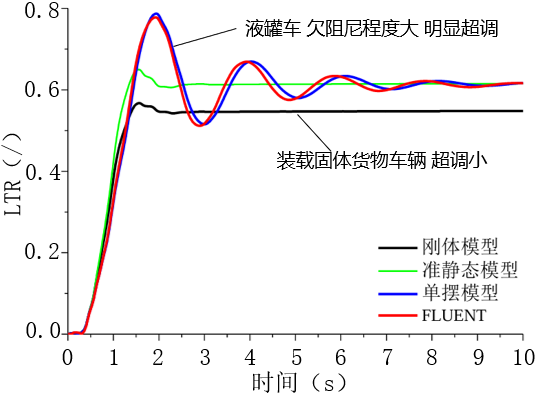
\includegraphics[width=0.92\linewidth]{fig/chap3/ltr_feature.png}}\\
  \subfloat[Solid-cargo and liquid-cargo reference comparison\label{fig:traj_compare_journal}]
    {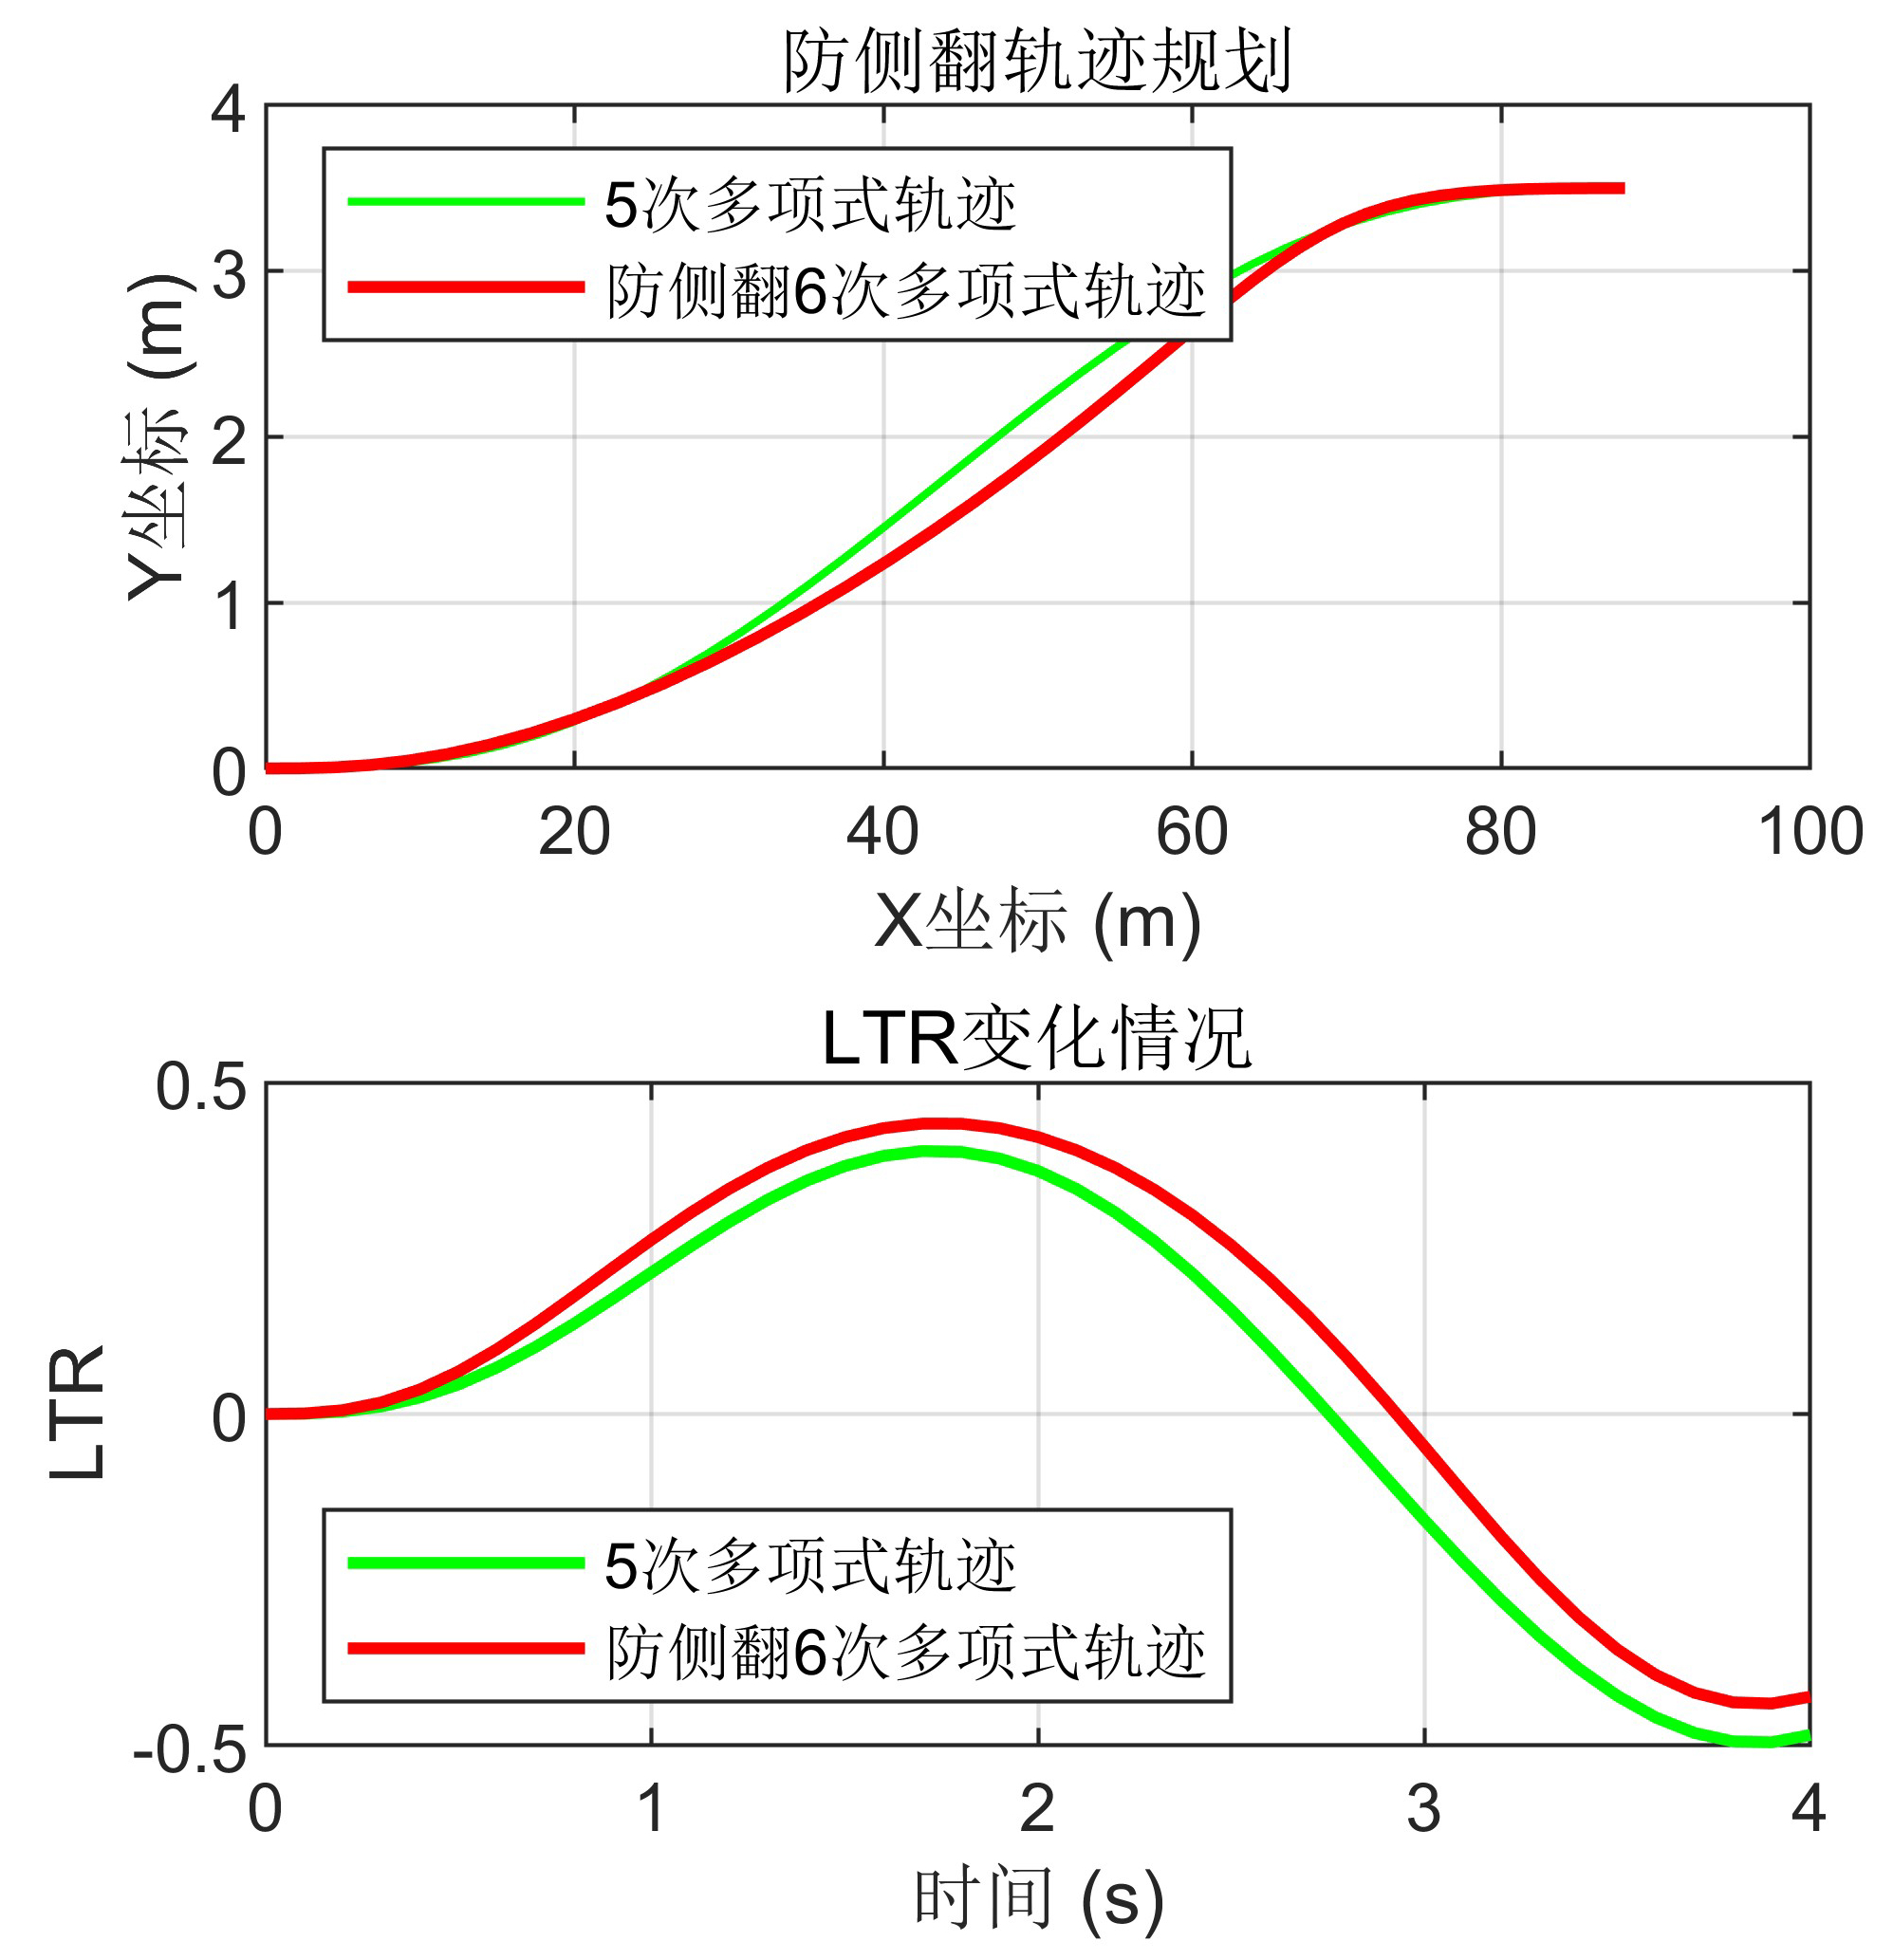
\includegraphics[width=0.92\linewidth]{fig/chap3/liquid_traj.jpg}}
  \caption{Rollover-aware lane-change reference generation on the cloud side.}
  \label{fig:cloud_rollover_reference}
\end{figure}
